Thinking...
The user wants a translation of a Japanese sentence into English, preserving TeX code as is. The Japanese text: "以下のの日本語文を英訳してください。ただしTeXのコードが挿入されているのでその部分はそのまま出力してください：" then the TeX figure environment.

We need to translate the Japanese sentence: "以下のの日本語文を英訳してください。ただしTeXのコードが挿入されているのでその部分はそのまま出力してください。" That translates to: "Please translate the following Japanese sentence into English. However, since there is TeX code inserted, output that part as is."

But perhaps the user wants the translation of the caption text? Actually the entire block includes TeX code with a caption in Japanese: "高被引用論文および新規出現高被引用論文の出現数". So they likely want the English translation of the Japanese caption, while keeping the TeX code unchanged. The instruction: "以下のの日本語文を英訳してください。ただしTeXのコードが挿入されているのでその部分はそのまま出力してください：" Then they give the figure environment with caption Japanese.

Thus we need to output the same TeX code but with the caption translated. So replace the Japanese caption with English translation, but keep everything else unchanged. Also maybe they want translation of the surrounding instruction? Probably just the figure code.

So translation: "Number of occurrences of highly cited papers and newly emerging highly cited papers". That seems appropriate.

Thus output:

\begin{figure}[h]
\begin{center}
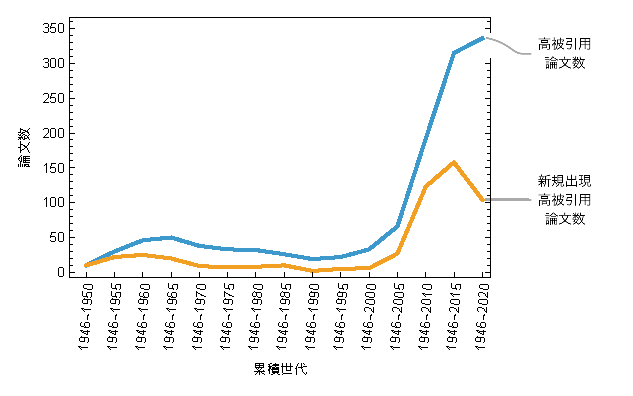
\includegraphics[width=76mm]{gr3.eps}
\caption{Number of occurrences of highly cited papers and newly emerging highly cited papers}
\label{fig:gr3}
\end{center}
\end{figure}

Make sure to keep the code unchanged except caption.
...done thinking.

\begin{figure}[h] 
\begin{center} 
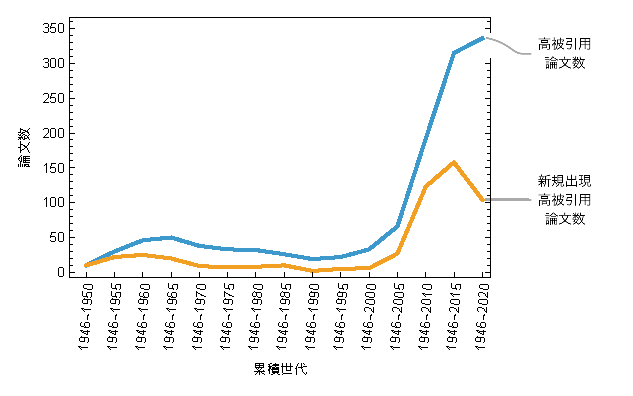
\includegraphics[width=76mm]{gr3.eps} 
\caption{Number of occurrences of highly cited papers and newly emerging highly cited papers} 
\label{fig:gr3} 
\end{center} 
\end{figure}

